\documentclass[nofonts]{ctexart}

% 设置中文字体
\setCJKmainfont{AR PL UMing CN}
\setCJKsansfont{AR PL UMing CN}
\setCJKmonofont{WenQuanYi Micro Hei Mono}

% 设置英文字体
\setmainfont{Times New Roman}
\setsansfont{Droid Sans Mono}
\setmonofont{FreeMono}

\usepackage{siunitx}
\usepackage{tikz}

\begin{document}
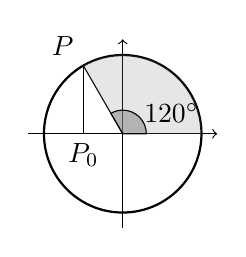
\begin{tikzpicture}
	\newcommand\iangle{120}

	% 画坐标轴
	\draw[->] (-1.2, 0) -- (1.2, 0);
	\draw[->] (0, -1.2) -- (0, 1.2);

	% 画圆
	\draw[thick] (0, 0) circle (1);

	% P 与 P0 两个点, 并连线
	\coordinate[label=\iangle: $P$] (P) at (\iangle: 1);
	\coordinate[label=below: $P_0$] (P0) at (P |- 0, 0);
	\draw (0, 0) -- (P);
	\draw (P) -- (P0);

	% 画大扇形
	\fill[fill=gray, fill opacity=0.2]
		(0, 0) -- (0: 1) arc (0: \iangle: 1) -- cycle;

	% 画角
	\filldraw[fill=gray, fill opacity=0.5]
		(0, 0) -- (0: 0.3) arc (0: \iangle: 0.3) -- cycle;

	% 画角的标识符
	\node[right] at (\iangle/2: 0.3) {\ang{\iangle}};
\end{tikzpicture}
\end{document}
